\section{Question 2}
\begin{enumerate}
  \item
    \begin{mytable}{val}{Table de différentes valeures des notes du test.}
      \begin{tabular}{ll}
        $n$                      & \np{252}\\
Moyenne                  & \np{1.059524e+01}\\
M\'ediane                & \np{1.050000e+01}\\
\'Ecart-type             & \np{2.642711e+00}\\
\'Etendue                & \np{1.250000e+01}\\
Coefficient de variation & \np{2.494244e-01}\\
Proportion de r\'eussite & \np{3.452381e-01}\\

      \end{tabular}
    \end{mytable}
  \item Utilisons la méthode des moments
    (qui donne la même chose que celle du maximum de vraissemblance pour
    une loi normale de toute façon).
    \begin{itemize}
      \item
        Pour la loi normale, on a
        \begin{align*}
          \bar{y} & = E(Y)\\
                  & = \mu\\
          \bar{y^2} & = E(Y^2)\\
                    & = \var(Y) + E(Y)^2\\
                    & = \sigma^2 + \mu^2
        \end{align*}
        ce qui donne
        \begin{align*}
          \mu & = \bar{y}\\
          \sigma^2 & = \bar{y^2} - \bar{y}^2.
        \end{align*}
      \item
        Pour la loi de Weibull, on a
        \begin{align*}
          \bar{y} & = E(Y)\\
                  & = \sqrt[m]{\alpha}\Gamma\left(1 + \frac{1}{m}\right)\\
          \bar{y^2} & = E(Y^2)\\
                    & = \var(Y) + E(Y)^2\\
                    & = \alpha^{2/m}\left(\Gamma\left(1 + \frac{2}{m}\right) -
                    \Gamma^2\left(1 + \frac{1}{m}\right)\right) + \alpha^{2/m}\Gamma^2\left(1 + \frac{1}{m}\right)\\
                    & = \alpha^{2/m}\Gamma\left(1 + \frac{2}{m}\right)
        \end{align*}
        ce qui donne
        \begin{align*}
          \mu & = \bar{y}\\
          \sigma^2 & = \bar{y^2} - \bar{y}^2.
        \end{align*}
    \end{itemize}
  \item
    La figure~\ref{fig:distrib} donne quelques exemple de distribution normale et de Weibull.
    On remarque que la distribution de Weibull a $f(x; \alpha, m) = 0$ $\forall x \leq 0$
    ce qui a du sens dans ce cas car une note ne peut pas être négative alors que
    la distribution normale a $f(x) > 0$ pour $f \leq 0$ même si la valeur est très faible
    si $\mu > 0$ et que $\sigma^2$ est suffisamment petit.

    \begin{figure}
      \centering
      \begin{subfigure}[b]{0.45\textwidth}
        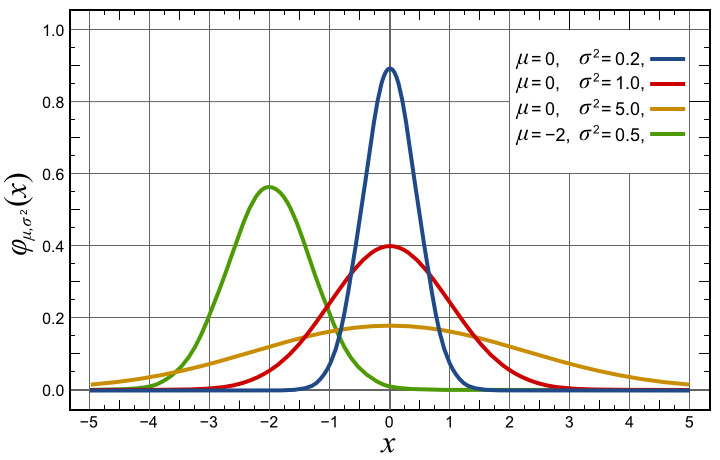
\includegraphics[width=\textwidth]{img/normal.png}
        \caption{Normal distribution}
        \label{fig:normal}
      \end{subfigure}%
      ~ %add desired spacing between images, e. g. ~, \quad, \qquad etc.
      %(or a blank line to force the subfigure onto a new line)
      \begin{subfigure}[b]{0.45\textwidth}
        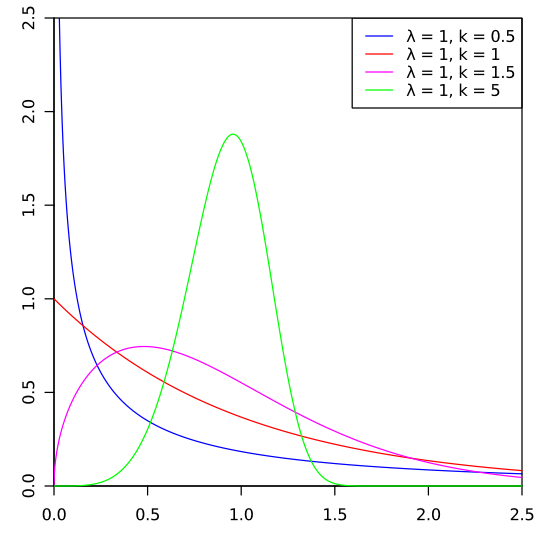
\includegraphics[width=\textwidth]{img/weibull}
        \caption{Weibull distribution}
        \label{fig:weibull}
      \end{subfigure}
      \caption{Comparison for Weibull and Normal distributions}
      \label{fig:distrib}
    \end{figure}
    De plus, la distribution normale est symétrique autour de $\mu$ alors que la distribution
    des notes d'un test n'est pas spécialement symétrique.
  \item
    La moyenne vaut 11.65, je ne pense donc pas qu'il réussira son examen.
  \item
\end{enumerate}
